\documentclass{beamer}
\mode<presentation>{
  \usetheme{Boadilla}
  \usefonttheme[onlylarge]{structurebold}
  \usefonttheme[stillsansseriflarge]{serif}
  \setbeamerfont*{frametitle}{size=\normalsize,series=\bfseries}
  % \setbeamertemplate{navigation symbols}{}
  \setbeamercovered{transparent}
}
\usepackage[english]{babel}
\usepackage[latin1]{inputenc}
\usepackage{times}
\usepackage[T1]{fontenc}
\usepackage{amsmath}
\usepackage{amssymb}
\usepackage{esint}
\usepackage{hyperref}
\usepackage{tikz}
\usepackage{xkeyval}
\usepackage{xargs}
\usepackage{verbatim}
\usepackage{listings}
\usepackage{multimedia}
\usetikzlibrary{
  arrows,
  calc,
  decorations.pathmorphing,
  decorations.pathreplacing,
  decorations.markings,
  fadings,
  positioning,
  shapes
}

\mode<handout>{
  \usepackage{pgfpages}
  \pgfpagesuselayout{4 on 1}[a4paper,landscape,border shrink=5mm]
  \setbeamercolor{background canvas}{bg=black!10}
}

\newcommand\pgfmathsinandcos[3]{%
  \pgfmathsetmacro#1{sin(#3)}%
  \pgfmathsetmacro#2{cos(#3)}%
}
\newcommand\LongitudePlane[3][current plane]{%
  \pgfmathsinandcos\sinEl\cosEl{#2} % elevation
  \pgfmathsinandcos\sint\cost{#3} % azimuth
  \tikzset{#1/.estyle={cm={\cost,\sint*\sinEl,0,\cosEl,(0,0)}}}
}
\newcommand\LatitudePlane[3][current plane]{%
  \pgfmathsinandcos\sinEl\cosEl{#2} % elevation
  \pgfmathsinandcos\sint\cost{#3} % latitude
  \pgfmathsetmacro\yshift{\cosEl*\sint}
  \tikzset{#1/.estyle={cm={\cost,0,0,\cost*\sinEl,(0,\yshift)}}} %
}
\newcommand\DrawLongitudeCircle[2][1]{
  \LongitudePlane{\angEl}{#2}
  \tikzset{current plane/.prefix style={scale=#1}}
  % angle of "visibility"
  \pgfmathsetmacro\angVis{atan(sin(#2)*cos(\angEl)/sin(\angEl))} %
  \draw[current plane] (\angVis:1) arc (\angVis:\angVis+180:1);
  \draw[current plane,dashed] (\angVis-180:1) arc (\angVis-180:\angVis:1);
}
\newcommand\DrawLatitudeCircleArrow[2][1]{
  \LatitudePlane{\angEl}{#2}
  \tikzset{current plane/.prefix style={scale=#1}}
  \pgfmathsetmacro\sinVis{sin(#2)/cos(#2)*sin(\angEl)/cos(\angEl)}
  % angle of "visibility"
  \pgfmathsetmacro\angVis{asin(min(1,max(\sinVis,-1)))}
  \draw[current plane,decoration={markings, mark=at position 0.6 with {\arrow{<}}},postaction={decorate},line width=.6mm] (\angVis:1) arc (\angVis:-\angVis-180:1);
  \draw[current plane,dashed,line width=.6mm] (180-\angVis:1) arc (180-\angVis:\angVis:1);
}
\newcommand\DrawLatitudeCircle[2][1]{
  \LatitudePlane{\angEl}{#2}
  \tikzset{current plane/.prefix style={scale=#1}}
  \pgfmathsetmacro\sinVis{sin(#2)/cos(#2)*sin(\angEl)/cos(\angEl)}
  % angle of "visibility"
  \pgfmathsetmacro\angVis{asin(min(1,max(\sinVis,-1)))}
  \draw[current plane] (\angVis:1) arc (\angVis:-\angVis-180:1);
  \draw[current plane,dashed] (180-\angVis:1) arc (180-\angVis:\angVis:1);
}
\newcommand\coil[1]{
  {\rh * cos(\t * pi r)}, {\apart * (2 * #1 + \t) + \rv * sin(\t * pi r)}
}
\makeatletter
\define@key{DrawFromCenter}{style}[{->}]{
  \tikzset{DrawFromCenterPlane/.style={#1}}
}
\define@key{DrawFromCenter}{r}[1]{
  \def\@R{#1}
}
\define@key{DrawFromCenter}{center}[(0, 0)]{
  \def\@Center{#1}
}
\define@key{DrawFromCenter}{theta}[0]{
  \def\@Theta{#1}
}
\define@key{DrawFromCenter}{phi}[0]{
  \def\@Phi{#1}
}
\presetkeys{DrawFromCenter}{style, r, center, theta, phi}{}
\newcommand*\DrawFromCenter[1][]{
  \setkeys{DrawFromCenter}{#1}{
    \pgfmathsinandcos\sint\cost{\@Theta}
    \pgfmathsinandcos\sinp\cosp{\@Phi}
    \pgfmathsinandcos\sinA\cosA{\angEl}
    \pgfmathsetmacro\DX{\@R*\cost*\cosp}
    \pgfmathsetmacro\DY{\@R*(\cost*\sinp*\sinA+\sint*\cosA)}
    \draw[DrawFromCenterPlane] \@Center -- ++(\DX, \DY);
  }
}
\newcommand*\DrawFromCenterText[2][]{
  \setkeys{DrawFromCenter}{#1}{
    \pgfmathsinandcos\sint\cost{\@Theta}
    \pgfmathsinandcos\sinp\cosp{\@Phi}
    \pgfmathsinandcos\sinA\cosA{\angEl}
    \pgfmathsetmacro\DX{\@R*\cost*\cosp}
    \pgfmathsetmacro\DY{\@R*(\cost*\sinp*\sinA+\sint*\cosA)}
    \draw[DrawFromCenterPlane] \@Center -- ++(\DX, \DY) node {#2};
  }
}
\makeatother

% not mandatory, but I though it was better to set it blank
\setbeamertemplate{headline}{}
\def\beamer@entrycode{\vspace{-\headheight}}

\tikzstyle{snakearrow} = [decorate, decoration={pre length=0.2cm,
  post length=0.2cm, snake, amplitude=.4mm,
  segment length=2mm},thick, ->]

%% document-wide tikz options and styles

\tikzset{%
  % >=latex, % option for nice arrows
  inner sep=0pt,%
  outer sep=2pt,%
  mark coordinate/.style={inner sep=0pt,outer sep=0pt,minimum size=3pt,
    fill=black,circle}%
}
\tikzset{
  % Define standard arrow tip
  >=stealth',
  % Define style for boxes
  punkt/.style={
    rectangle,
    rounded corners,
    draw=black, very thick,
    text width=8em,
    minimum height=2.5em,
    text centered},
}
\makeatletter
\newbox\@backgroundblock
\newenvironment{backgroundblock}[2]{%
  \global\setbox\@backgroundblock=\vbox\bgroup%
  \unvbox\@backgroundblock%
  \vbox to0pt\bgroup\vskip#2\hbox to0pt\bgroup\hskip#1\relax%
}{\egroup\egroup\egroup}
\addtobeamertemplate{background}{\box\@backgroundblock}{}
\makeatother

\title{Function multiversioning in system image}
\subtitle{All about vector registers}
\date{Oct. 16, 2017}
\author{Yichao Yu}
\institute{Harvard}

\begin{document}

\begin{frame}{}
  \titlepage
\end{frame}

\begin{frame}{}
  \begin{center}
    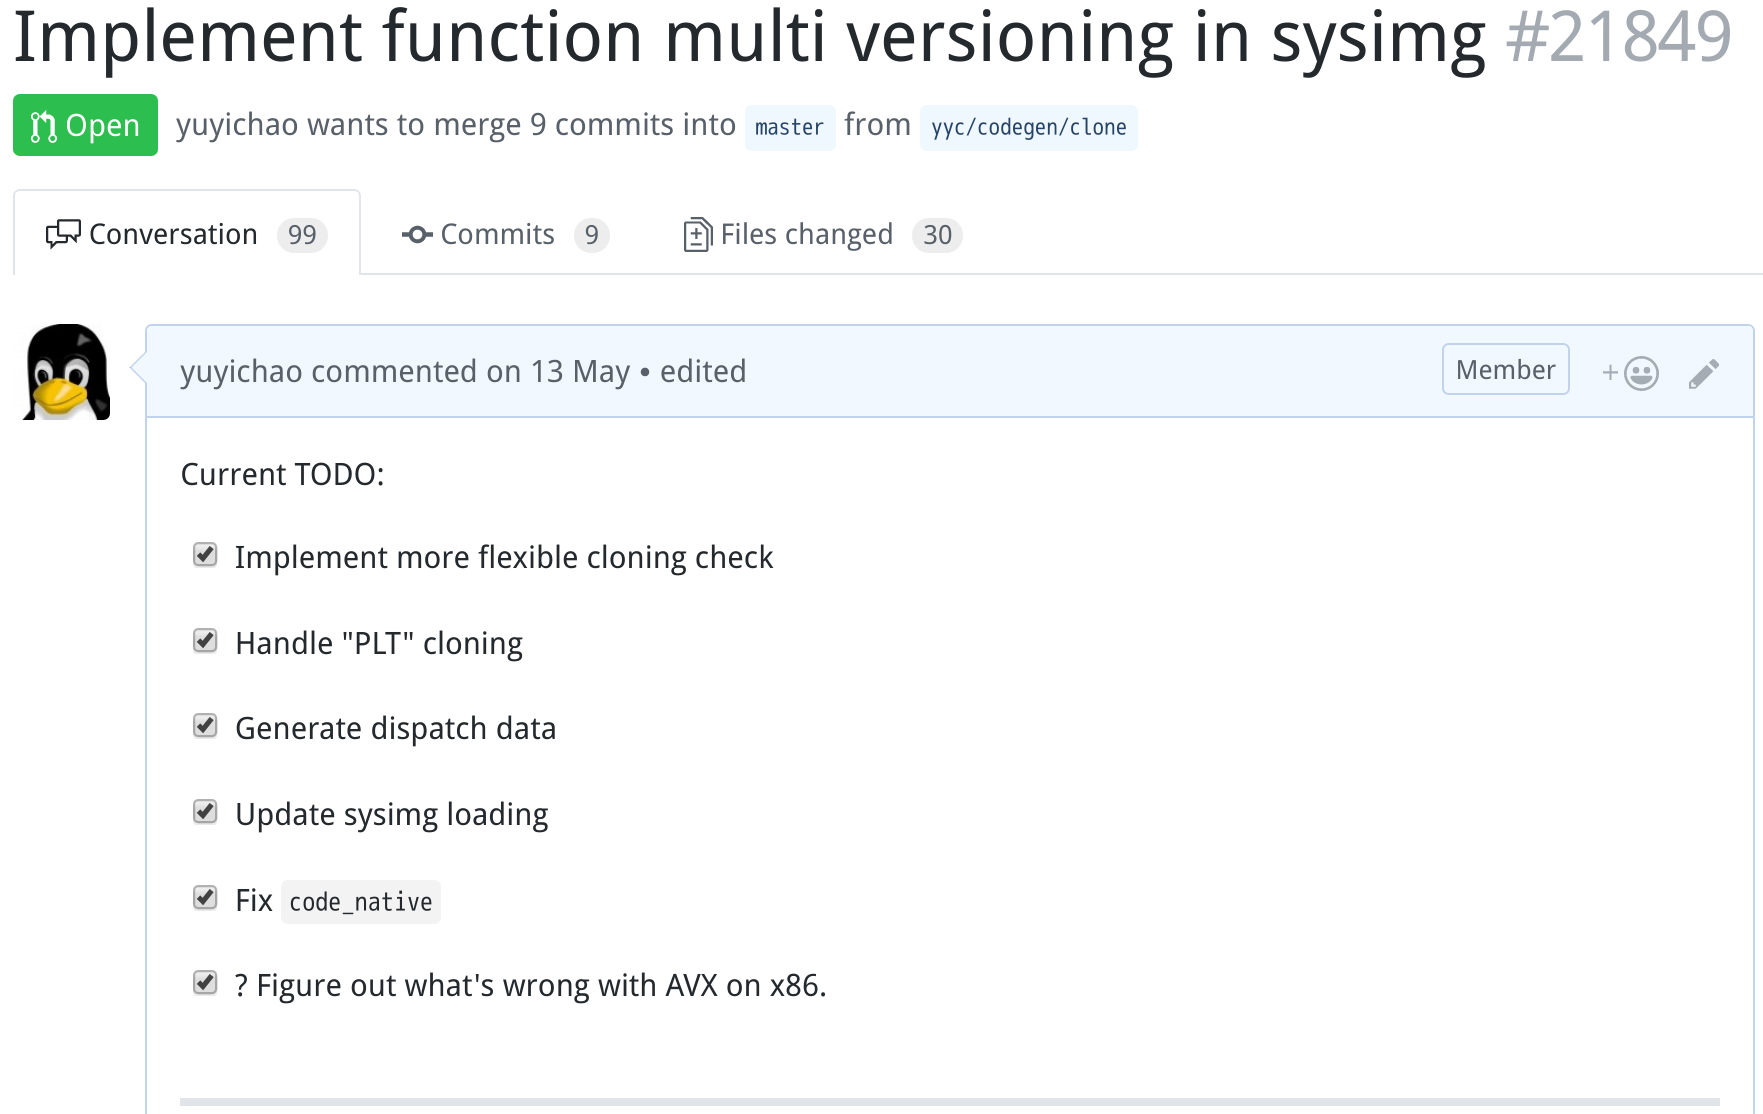
\includegraphics[width=11cm]{imgs/pr21849.png}
  \end{center}
\end{frame}

% Probably more techincal and low level than many other talks
% So let's set the base line
% By Jameson

% With that in mind, feel free to ask questions.

% I'll talk less about this PR specifically,
% but more about the general issue when dealing with code compiled for different architectures.

\begin{frame}{Goal}
  \visible<+-> {
    \begin{block}{Amount of implementation details}
      \begin{itemize}
      \item<+-> Just enough to make Jeff happy
      \item<+-> Without losing the audience
      \item<+-> With a single version of the talk \textbf{(Important!)}
      \end{itemize}
    \end{block}
  }
\end{frame}

% Story
% * openlibm performance issue

\begin{frame}{How did it all begin}
  \begin{tikzpicture}
    \node at (0, 0) {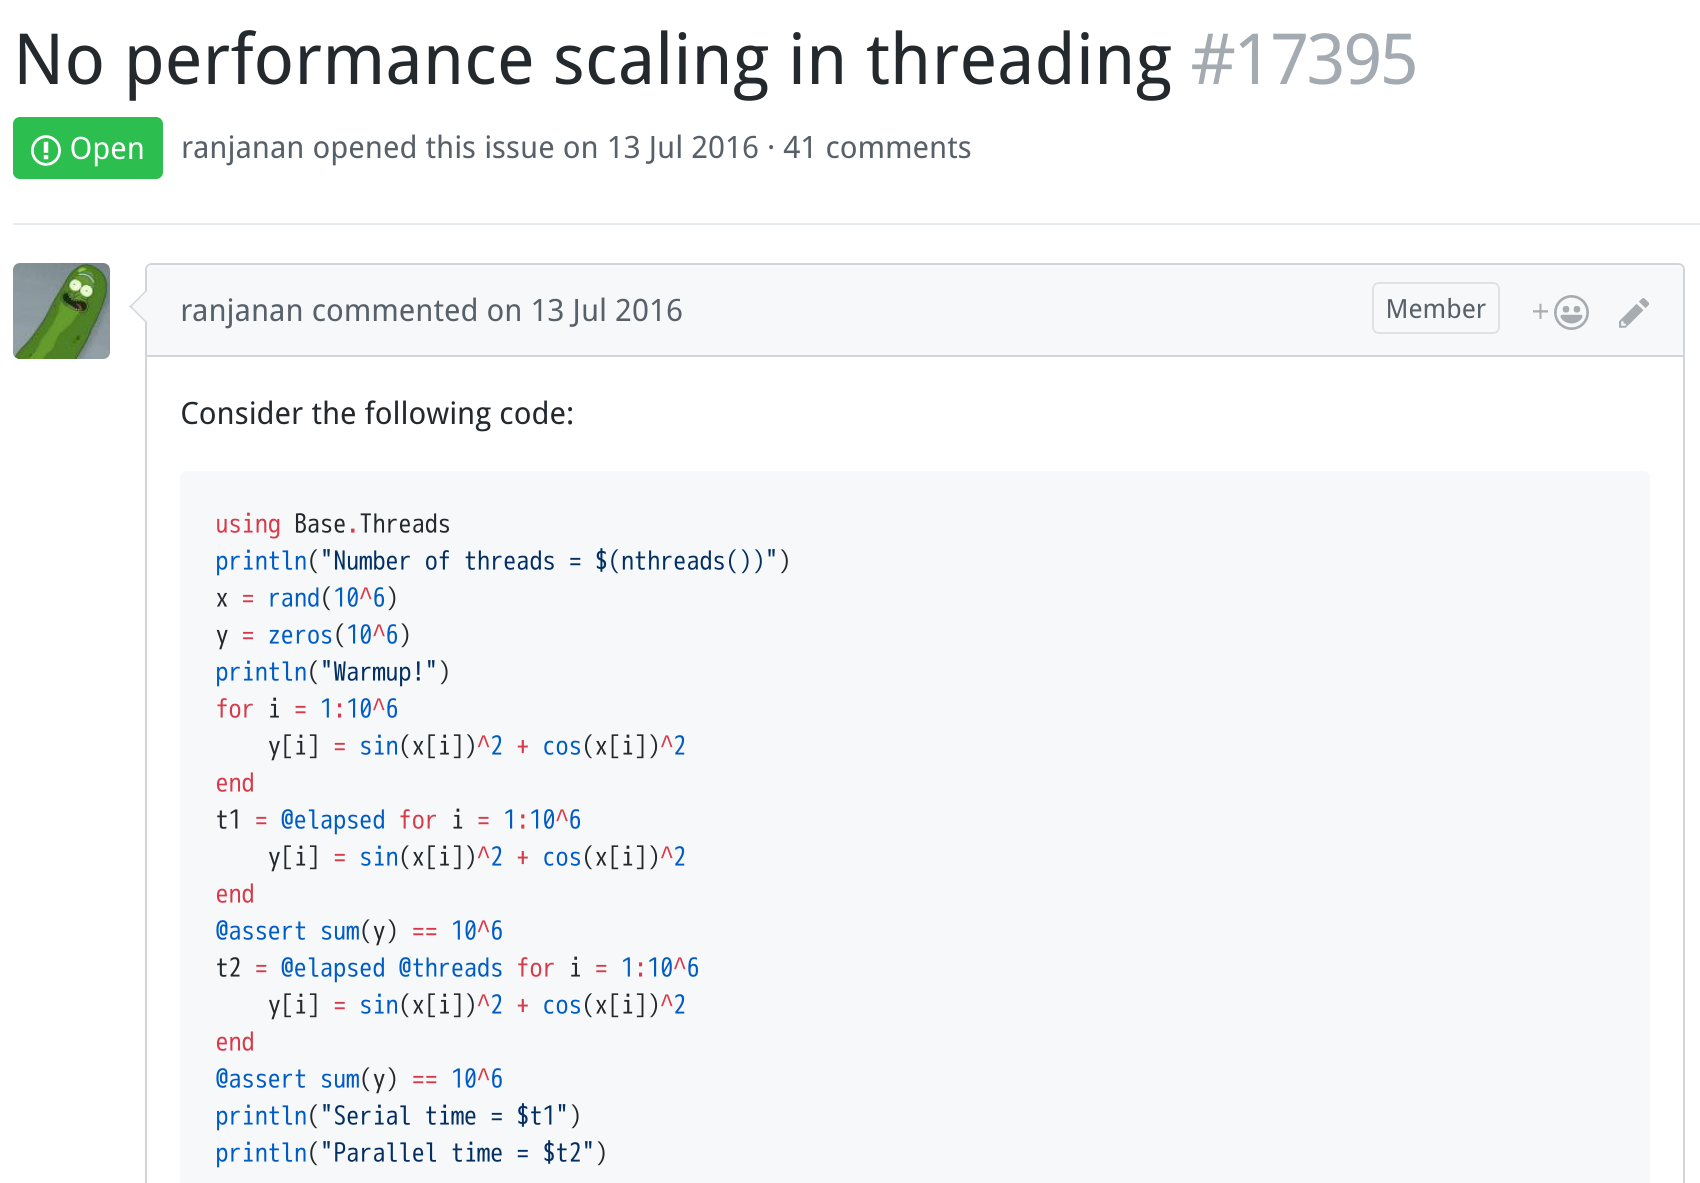
\includegraphics[width=11cm]{imgs/issue17395.png}};
    \visible<2>{
      \fill[white,opacity=0.85] (5.5, 3.9) rectangle (-5.5, -3.9);
      \node[fill=red!20!white,thick,rounded corners=.3cm,inner sep=8pt] at (-4, 2) (S1) {Startup};
      \node[fill=red!20!white,thick,rounded corners=.3cm,inner sep=8pt] at (2, 2) (S2) {Slow loop};

      \node[fill=green!20!white,thick,rounded corners=.3cm,inner sep=8pt] at (-4, -2) (F2) {Magic};
      \node[fill=green!20!white,thick,rounded corners=.3cm,inner sep=8pt] at (2, -2) (F3) {Fast loop};
      \draw[->, line width=1.4] (S1) edge (S2) (S2) edge (F2) (F2) edge (F3);

      \node at (3, 0) (L0) {Same code};

      \draw[->, gray, line width=1] (L0) edge (S2);
      \draw[->, gray, line width=1] (L0) edge (F3);

      \draw[<-, line width=1.4] (S2.north) arc(190:-80:0.9);
      \draw[<-, line width=1.4] (F3.south) arc(-190:80:0.9);
    }
  \end{tikzpicture}
\end{frame}

\begin{frame}{Register size}
  \begin{center}
    \begin{tikzpicture}
      \node at (-4, 2) (ax) {\textbf{ax}};
      \node at (-2, 2) (eax) {\textbf{eax}};
      \node at (0, 2) (rax) {\textbf{rax}};

      \node at (0, 1.3) (mmx0) {\textbf{mmx0}};
      \node at (2, 1.3) (xmm0) {\textbf{xmm0}};
      \node at (4, 1.3) (ymm0) {\textbf{ymm0}};
      \node at (6, 1.3) (zmm0) {\textbf{zmm0}};

      \draw[->, line width=1, gray] (ax) edge (eax);
      \draw[->, line width=1, gray] (eax) edge (rax);
      \draw[->, line width=1, gray] (mmx0) edge (xmm0);
      \draw[->, line width=1, gray] (xmm0) edge (ymm0);
      \draw[->, line width=1, gray] (ymm0) edge (zmm0);

      \visible<2-> {
        \node[right] at (-4, 0) (A) {More/larger registers};
        \node[right] at (2, 0) (B) {More states to manage};
        \draw[->, line width=1, gray] (A) edge (B);
      }
      \visible<3-> {
        \node[right] at (-4, -0.7) {(Intel got something wrong almost everytime)};
      }
    \end{tikzpicture}
  \end{center}
\end{frame}

\end{document}
